\large
	\def\imbcircle{(-210:2) circle (2.725cm)}
	\def\dscircle{(-330:2) circle (2.725cm)}
	\def\mdcircle{(-90:2) circle (2.725cm)}

	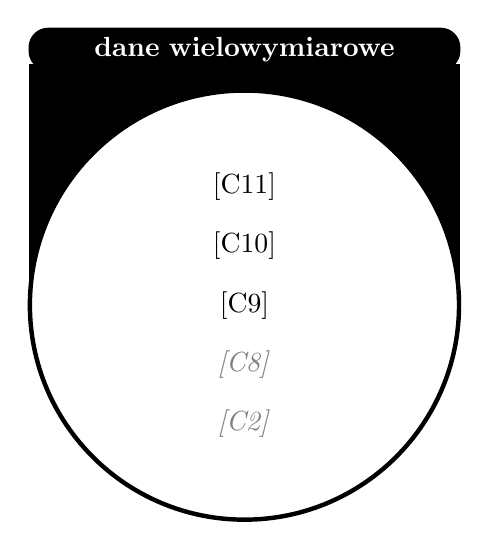
\begin{tikzpicture}
      	
      	\node[fill=black,rotate=0, text width=5.25cm, text height=2.9cm] at (90:-.5) {};
		\node[color=white,fill=black,rotate=0,rounded corners=.25cm, text width=5.25cm, align=center] at (90:1.25) {\bfseries \textsc{dane wielowymiarowe}};
      	
      	\draw[fill=white] \mdcircle;
      	\draw[ultra thick] \mdcircle;
      	
      	% 10 9 11 
      	% MD
      	\node at (-90:.5) {[C11]};
      	\node at (-90:1.25) {[C10]};    
      	\node at (-90:2.0) {[C9]};
      	%\node at (-330-180:1.75) {[4]};
      	      	   
      	\node at (-90:2.75) {\color{black!50}\emph{[C8]}};   
      	\node at (-90:3.5) {\color{black!50}\emph{[C2]}};
      	% DS + MD
      	%\node at (-210-180:1.25) {[5]};
      	%\node at (-210-180:1.75) {[6]};
      	
      	% ALL
      	%\node at (0:0) {[7]};
	\end{tikzpicture}